\subsection{Modes}

Die loolou Erweiterung hat vier verschiedene Modi zum Spielen. Diese k"onnen w"ahrend dem Spiel einfach "uber den Drucktaster am Oberteil der Spielbasis umgeschaltet werden.
Die vier roten LEDs neben dem Drucktaster zeigen dabei den aktuellen Modus an. \\
Die folgende Tabelle beschreibt die 4 verschiedenen Modi.

\vspace{1cm}
\begin{table}[ht]
	\centering

	\begin{tabular}{ c | p{8cm} } 
		% table header
		Modus								& Beschreibung \\ 
		\hline \hline
		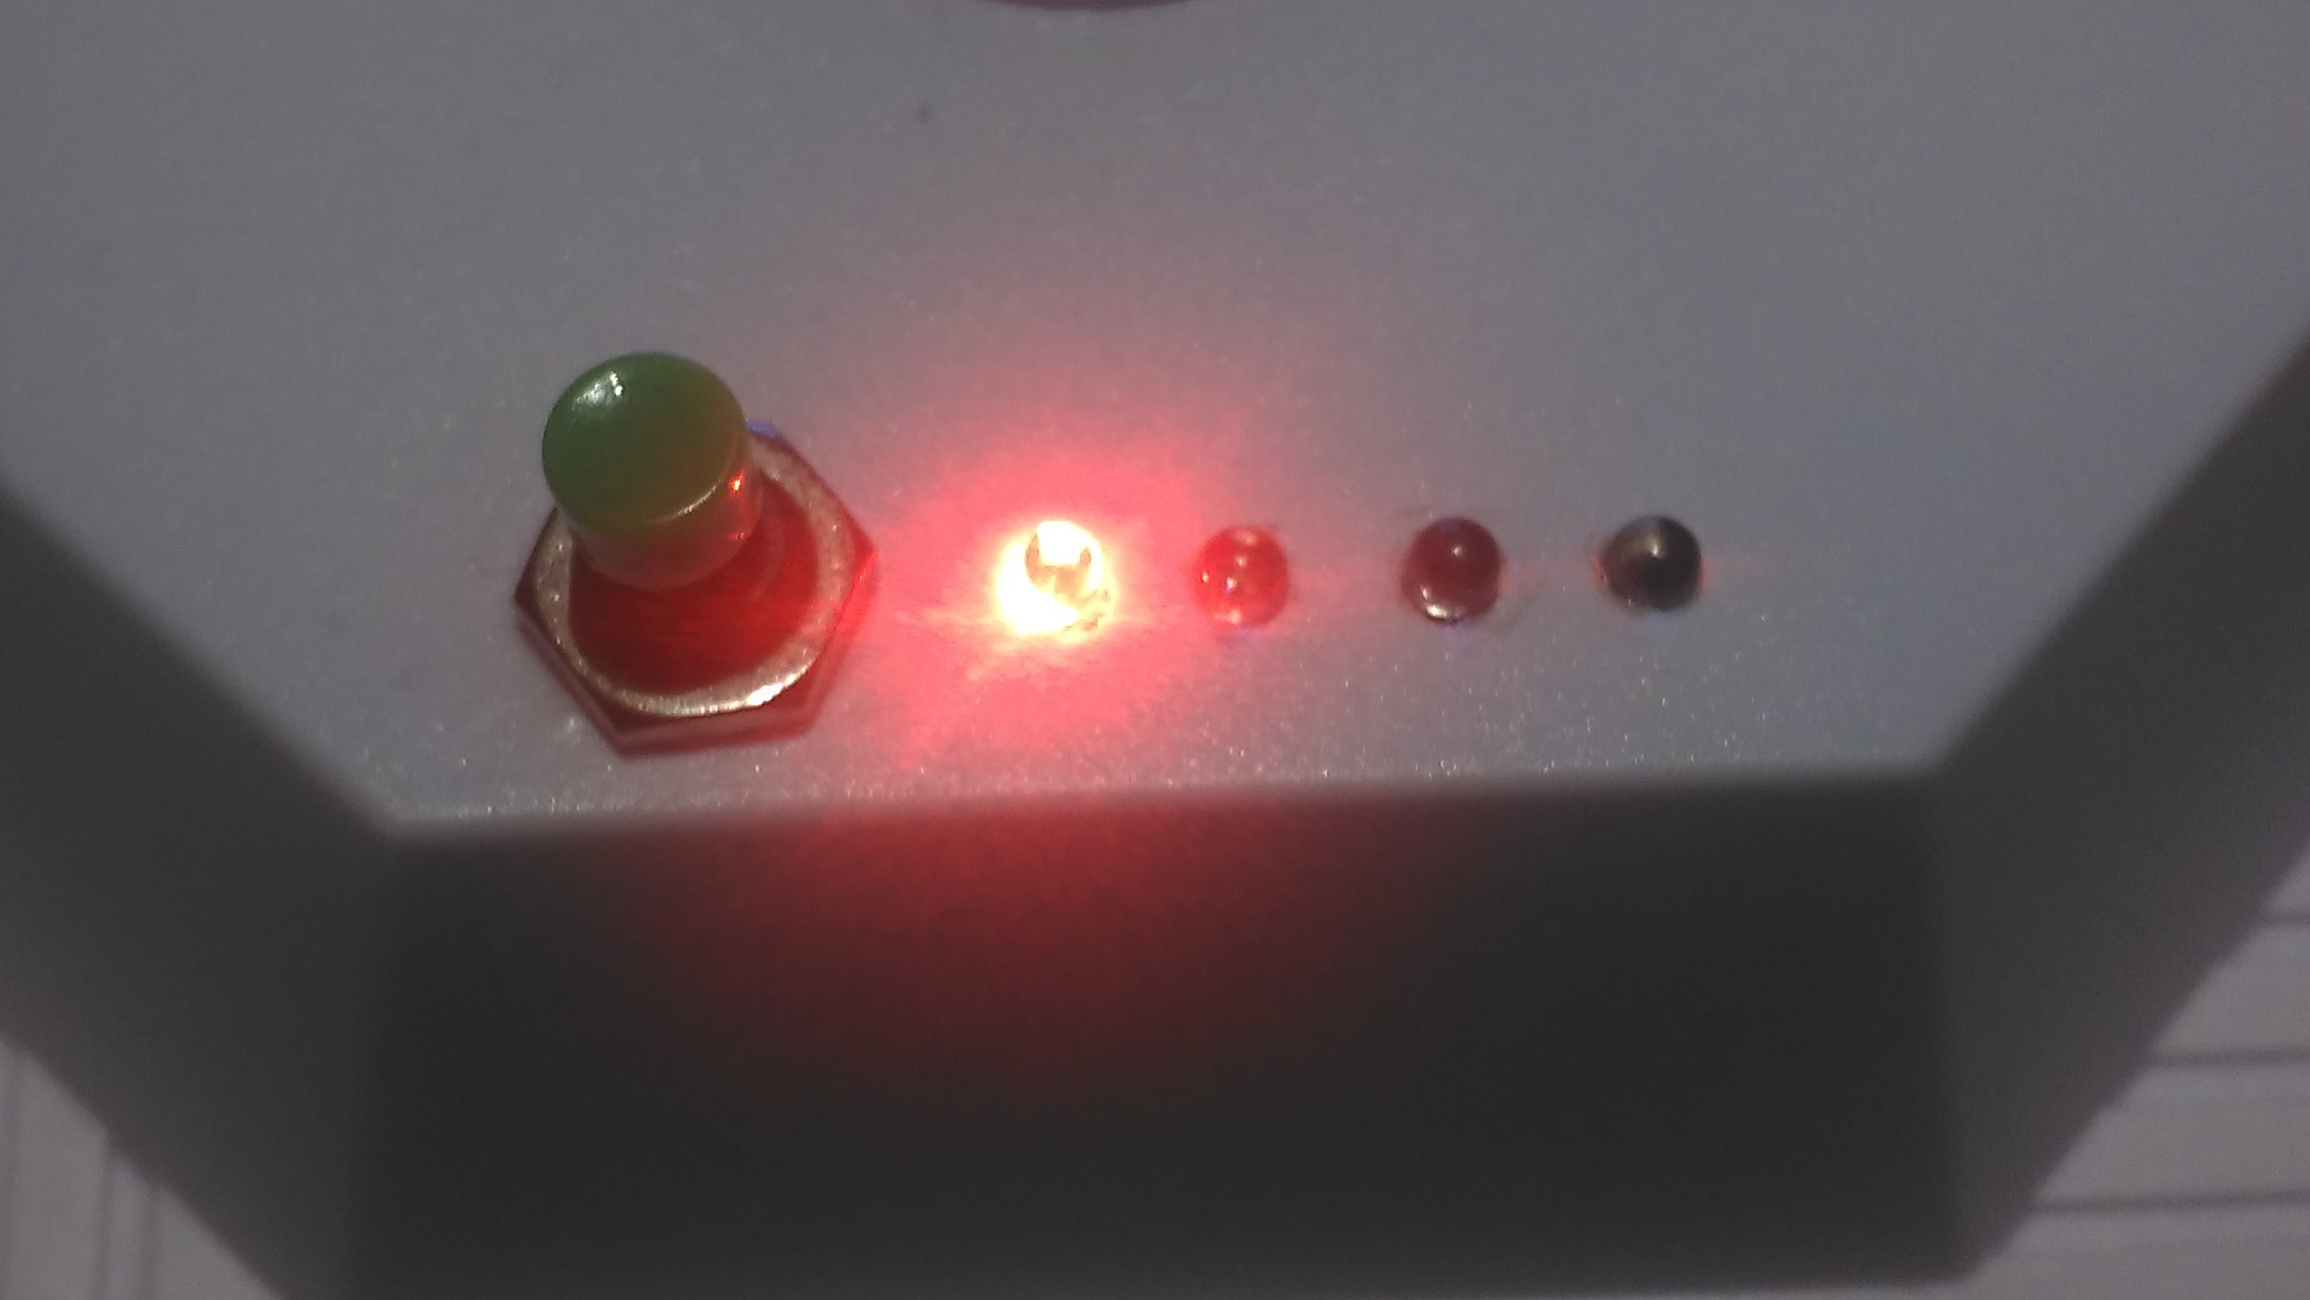
\includegraphics[width=0.2\textwidth]{pictures/mode_1.jpg}	& Einfacher Modus.\newline Looping Louie dreht sich so schnell wie beim originalen Spiel.  \\
		\hline
		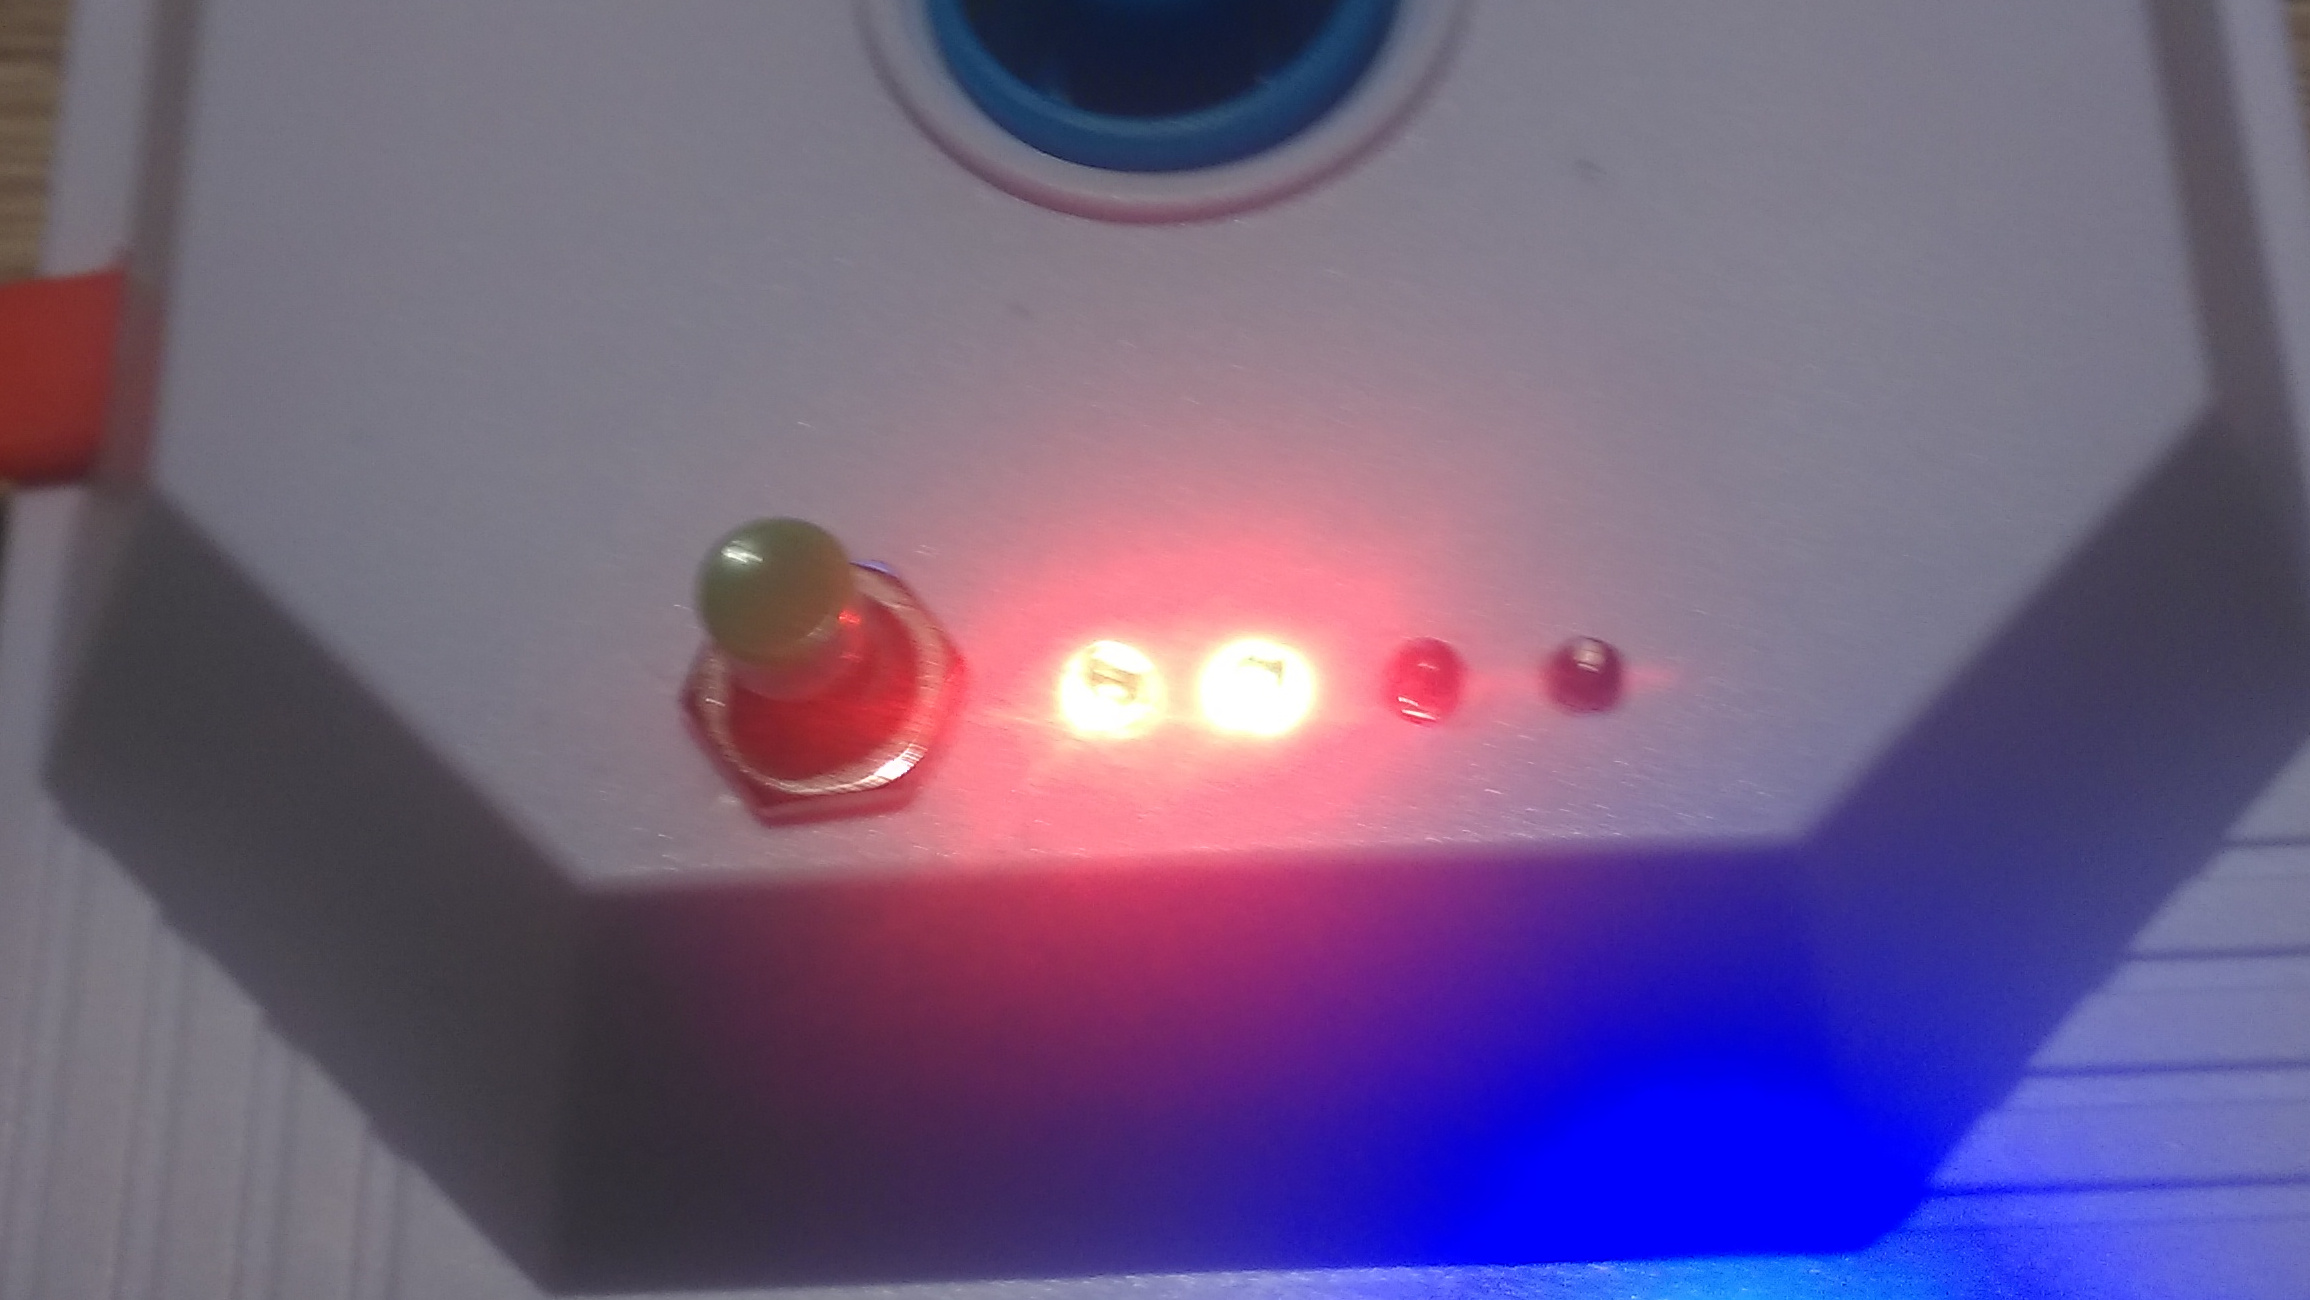
\includegraphics[width=0.2\textwidth]{pictures/mode_2.jpg}	& Schneller Modus.\newline Looping Louie dreht sich viel schneller als gewohnt. \\
		\hline
		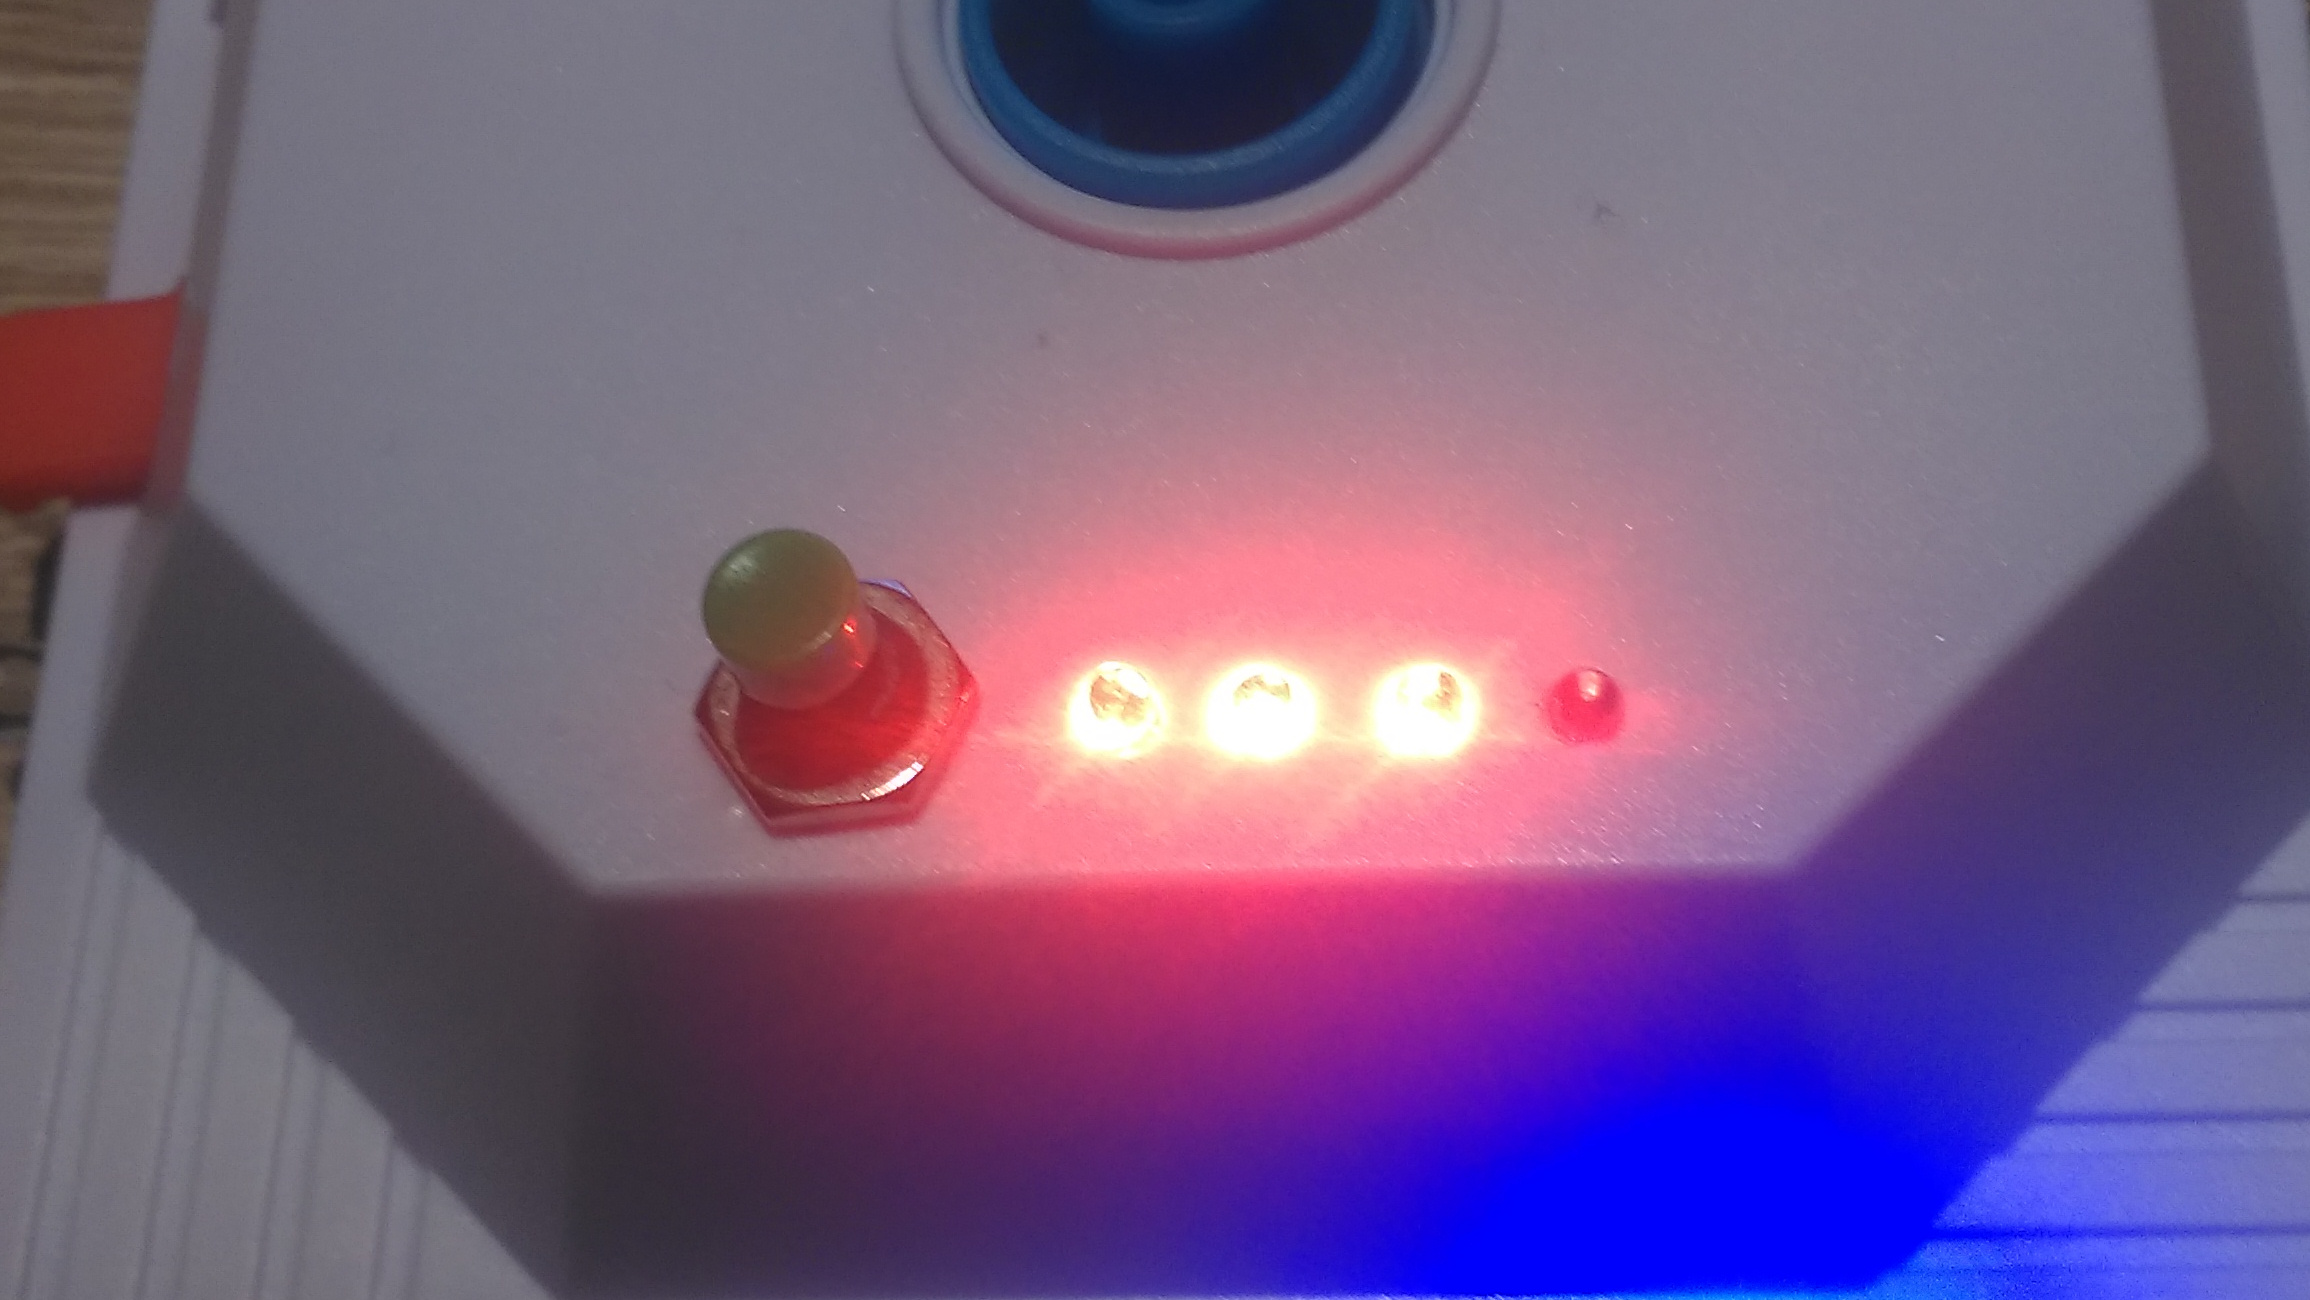
\includegraphics[width=0.2\textwidth]{pictures/mode_3.jpg}	& Zuf"alliger Modus.\newline Looping Louie "andert seine Gewschwindigkeit und bleibt auch mal stehen. \\
		\hline
		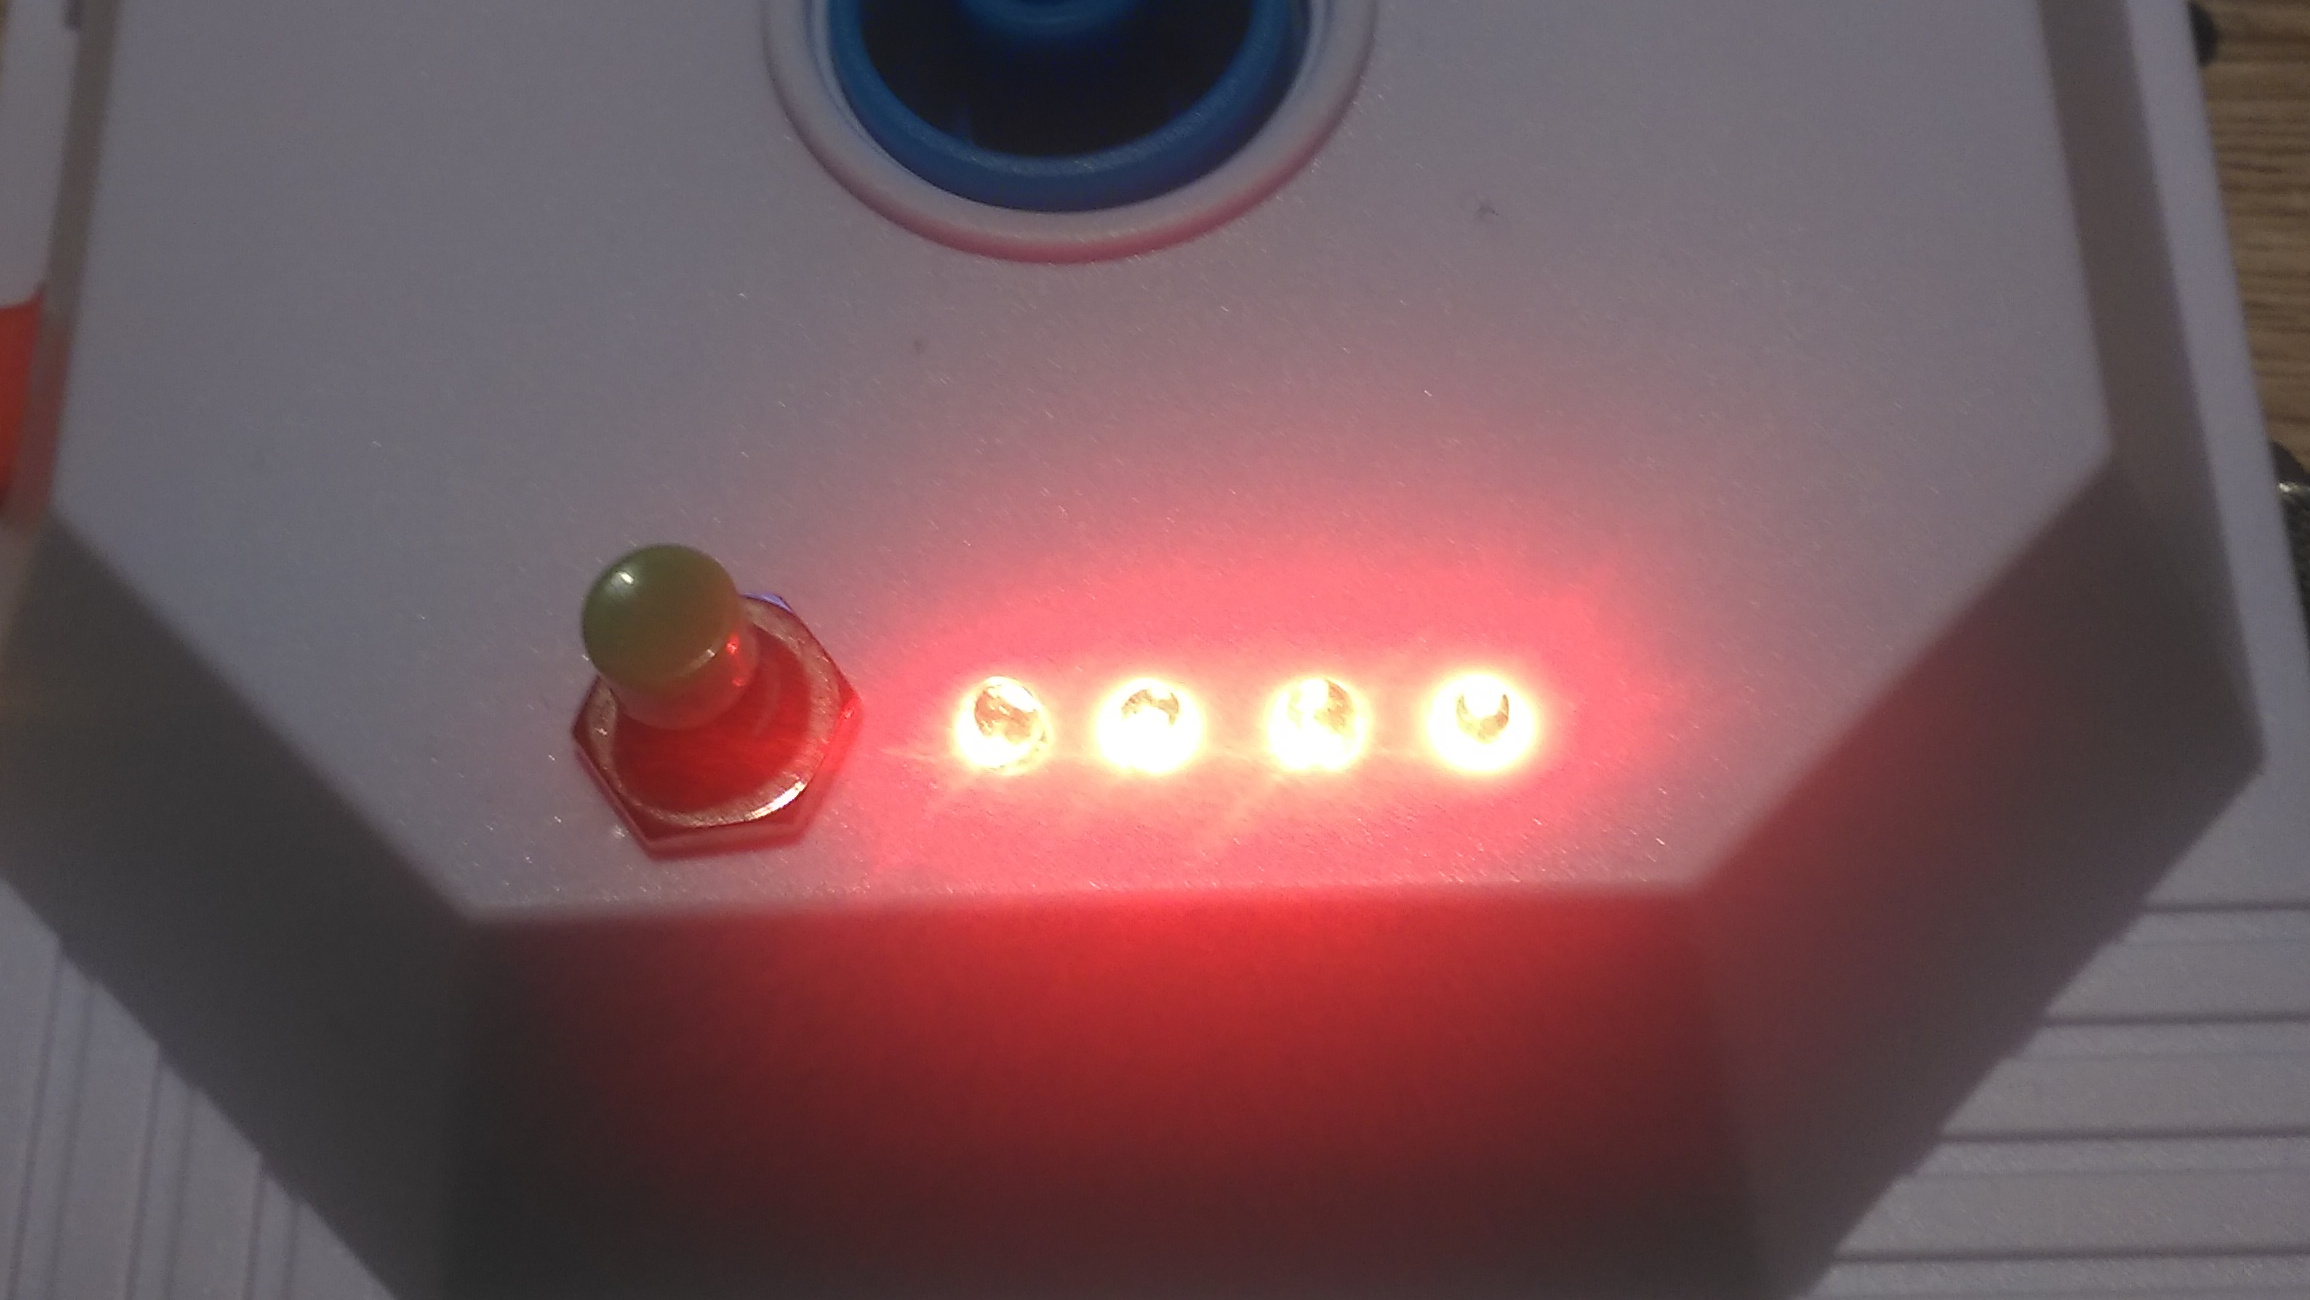
\includegraphics[width=0.2\textwidth]{pictures/mode_4.jpg}	& Zuf"alliger Modus mit R"uckw"artsgang.\newline Looping Louie "andert seine Geschwindigkeit und Richtung. \\
		\hline
	\end{tabular}

	\caption{Spielmodi}
	\label{table:mode}
\end{table}
\vspace{0.5cm}

\subsection{Source code}
tbd % TODO
\subsubsection{Github}

tbd % TODO
\href{https://github.com/}{https://github.com/}
\vspace{0.5cm}

\subsubsection{Defines}
\begin{lstlisting}[caption={Defines},label=lst:defines]
// ********************************************************
// PWM values
// ********************************************************
#define PWM_OFF   0 // 0V ( OFF )
#define PWM_3V   85 // 3V ( (9V / 255) * 85 = 3V )
#define PWM_9V  255 // 9V


// ********************************************************
// PWM values
// ********************************************************
//
//   1000000Hz ( F_CPU )
//  --------------------- = 976,56 ( 0x3D0 )
//   1024 * 1Hz (1 sec)
#define TIMER_INT_DEPLAY 0x3D0

// ********************************************************
// Pin description
// ********************************************************
//
//		  attiny 2313
//           ---------------------
//  RESET   -| 1 (PA2)  (VCC) 20 |- VCC
//  LED5    -| 2 (PD0)  (PB7) 19 |- SCK
//  LED6    -| 3 (PD1)  (PB6) 18 |- MISO
//  LED7    -| 4 (PA1)  (PB5) 17 |- MOSI
//  LED8    -| 5 (PA0)  (PB4) 16 |- FORWARD
//  BUTTON  -| 6 (PD2)  (PB3) 15 |- BACKWARD
//  NC      -| 7 (PD3)  (PB2) 14 |- PWM
//  LED1    -| 8 (PD4)  (PB1) 13 |- LED4
//  LED2    -| 9 (PD5)  (PB0) 12 |- LED3
//  GND     -| 10(GND)  (PD6) 11 |- NC
//           --------------------
//

// *** LEDs ***********************************************
#define PIN_LED1 PD4
#define PIN_LED2 PD5
#define PIN_LED3 PB0
#define PIN_LED4 PB1
#define PIN_LED5 PD0
#define PIN_LED6 PD1
#define PIN_LED7 PA1
#define PIN_LED8 PA0

#define PORT_LED1 PORTD
#define PORT_LED2 PORTD
#define PORT_LED3 PORTB
#define PORT_LED4 PORTB
#define PORT_LED5 PORTD
#define PORT_LED6 PORTD
#define PORT_LED7 PORTA
#define PORT_LED8 PORTA

#define DDR_LED1 DDRD
#define DDR_LED2 DDRD
#define DDR_LED3 DDRB
#define DDR_LED4 DDRB
#define DDR_LED5 DDRD
#define DDR_LED6 DDRD
#define DDR_LED7 DDRA
#define DDR_LED8 DDRA

// *** DIRECTION / PWM ************************************
#define PIN_DIRECTION_FORWARD  PB4
#define PIN_DIRECTION_BACKWARD PB3
#define PIN_PWM                PB2

#define PORT_DIRECTION_FORWARD  PORTB
#define PORT_DIRECTION_BACKWARD PORTB
//#define PORT_PWM

#define DDR_DIRECTION_FORWARD  DDRB
#define DDR_DIRECTION_BACKWARD DDRB
#define DDR_PWM                DDRB

#define REGISTER_PWM  OCR0A
#define MODE_PWM      (1 << COM0A1) | (1 << WGM00)
#define CLOCK_PWM     (1 << CS01)

#define REGISTER_TIMER OCR1A
#define MODE_TIMERA    0x00
#define MODE_TIMERB    (1 << WGM12) | (1 << CS12) | (1 << CS10)

// *** BUTTON *********************************************
#define PIN_BUTTON  PD2
#define PORT_BUTTON PORTD
#define DDR_BUTTON  DDRD
#define EDGE_TYPE_BUTTON (1 << ISC01)
\end{lstlisting}
\vspace{0.5cm}

\subsubsection{Main-Method}
\begin{lstlisting}[caption={Main-Method},label=lst:main]
// ****************************************************************************
// game
// ***************************************************************************/
int main(void) {

	setup();
	init();

	/* main loop */
	while (1) {
		/* all other uses interrupts */
		trigger_speed( speed );
		trigger_direction( direction );
		show_direction( direction );
		_delay_ms( 250 );
	}

	return 0;
}
\end{lstlisting}
\vspace{0.5cm}

\subsubsection{Setup-Method}
\begin{lstlisting}[caption={Setup-Method},label=lst:setup]
// ****************************************************************************
// setup system, set pin directions
// ***************************************************************************/
void setup( void )
{
	// leds
	GPIO_init( DDR_LED5, PIN_LED5, OUTPUT ); // 1
	GPIO_init( DDR_LED6, PIN_LED6, OUTPUT ); // 2
	GPIO_init( DDR_LED7, PIN_LED7, OUTPUT ); // 3
	GPIO_init( DDR_LED8, PIN_LED8, OUTPUT ); // 4

	GPIO_init( DDR_LED1, PIN_LED1, OUTPUT ); // red
	GPIO_init( DDR_LED2, PIN_LED2, OUTPUT ); // blue
	GPIO_init( DDR_LED3, PIN_LED3, OUTPUT ); // green
	GPIO_init( DDR_LED4, PIN_LED4, OUTPUT ); // yellow

	// motor control
	GPIO_init( DDR_DIRECTION_BACKWARD, PIN_DIRECTION_BACKWARD, OUTPUT ); // backward
	GPIO_init( DDR_DIRECTION_FORWARD,  PIN_DIRECTION_FORWARD,  OUTPUT ); // forward
	GPIO_init( DDR_PWM, PIN_PWM, OUTPUT ); // PWM
	PWM_enable( MODE_PWM, CLOCK_PWM, REGISTER_PWM, PWM_OFF );

	// button
	GPIO_init( DDR_BUTTON, PIN_BUTTON, INPUT);
	GPIO_interrupt( PORT_BUTTON, PIN_BUTTON, INT0, EDGE_TYPE_BUTTON );

	// timer interrupt
	TIMER_enable( MODE_TIMERA, MODE_TIMERB );

	// Enable interrupts
	sei();
}
\end{lstlisting}
\vspace{0.5cm}

\subsubsection{Init-Method}
\begin{lstlisting}[caption={Init-Method},label=lst:init]
// ****************************************************************************
// initialze syetem with default values
// ***************************************************************************/
void init( void )
{
	// set initial values
	active_led  = LED1;
	mode        = M_NORMAL_FORWARD;
	speed       = PWM_3V;
	direction   = FORWARD;

	// show current mode
	show_mode();

	// set seed
	init_random( TCNT1L );

	// initial pwm
	trigger_speed( PWM_3V );

	// set initial timer delay
	TIMER_set( TIMER_INT_DEPLAY );
}
\end{lstlisting}
\vspace{0.5cm}

\subsubsection{Interrupt Service Routine}
\begin{lstlisting}[caption={Interrupt Service Routine},label=lst:isr]
// ****************************************************************************
// interrupt service routine
// ***************************************************************************/
ISR(INT0_vect)
{
	ADD_ONE_BETWEEN( mode, M_NORMAL_FORWARD, M_RANDOM_RANDOM );
	show_mode();

	/* reset timer, call ISR to change speed/direction immediately */
	TIMER_reset();
	TIMER1_COMPA_vect();
}

ISR(TIMER1_COMPA_vect)
{
	direction = calc_direction();
	speed = calc_speed();
}
\end{lstlisting}
\vspace{0.5cm}

\subsubsection{Calculate direction}
\begin{lstlisting}[caption={Calculate direction},label=lst:calcdirection]
// ****************************************************************************
// calculates a new direction
// ***************************************************************************/
GameDirection calc_direction( void )
{
	switch( mode )
	{
		case M_NORMAL_FORWARD:
		case M_FAST_FORWARD:
		case M_RANDOM_FORWARD:
		default:
			return FORWARD;
			break;
		case M_RANDOM_RANDOM:
			return ( (get_random_between( 0, 10 ) == 0) ? BACKWARD : FORWARD ); /* 10% backward : 90% forward */
			break;
	}
}
\end{lstlisting}
\vspace{0.5cm}

\subsubsection{Calculate speed}
\begin{lstlisting}[caption={Calculate Speed},label=lst:calcspeed]
// ****************************************************************************
// calculates a new speed
// ***************************************************************************/
uint8_t calc_speed( void )
{
	switch( mode )
	{
	case M_NORMAL_FORWARD:
	default:
		return PWM_3V;
		break;
	case M_FAST_FORWARD:
		return PWM_9V;
		break;
	case M_RANDOM_FORWARD:
	case M_RANDOM_RANDOM:
	{
		/*
		 * Calculate speed in 25 steps.
		 * 0 = 0V, ...,  25 = ~9V
		 *
		 * For a better and faster playing pleasure,
		 * a probability of
		 * 10% values between   0V and 3,5V and
		 * 70% values between 3,5V and 6,0V is selected.
		 * 20% values between 7,0V and 9,0V is selected.
		 */
		static uint8_t r = 0;
		r = get_random_between( 0, 10 );
		if ( r == 0 )
		{ /* 20% slow ( 0V - ~3,5V ) */
			return get_random_between(  0, 100 );
		}
		else if ( r == 1 || r == 2 )
		{ /* 20% very fast /~7,0V - 9,0V */
			return get_random_between( 201, 255);
		}
		else
		{ /* 80% fast ( ~3,5V - ~7,0V ) */
			return get_random_between( 101, 200 );
		}
	}
		break;

	}
}
\end{lstlisting}
\vspace{0.5cm}

\subsection{How to compile}
\subsubsection{Build dependencies}
\begin{lstlisting}[caption={Build dependencies},language=sh,label=lst:builddep]
sudo apt-get install gcc-avr avrdude
\end{lstlisting}
\vspace{0.5cm}

\subsubsection{Compile}
\begin{lstlisting}[caption={Compile},language=sh,label=lst:makeall]
make
\end{lstlisting}
\vspace{0.5cm}

\subsubsection{Clean}
\begin{lstlisting}[caption={Clean},language=sh,label=lst:makeclean]
make clean
\end{lstlisting}
\vspace{0.5cm}

\subsubsection{Create documentation}
\begin{lstlisting}[caption={Create documentation},language=sh,label=lst:builddoc]
make doc
\end{lstlisting}
\vspace{0.5cm}


\subsection{How to program the Attiny2313}
tbd % TODO
\textbf{Der Strom darf nicht w"ahrend dem flashen eingesteckt sein.}

\subsubsection{Programming}
\begin{lstlisting}[caption={Programming},language=sh,label=lst:builddoc]
make burn
# or
make AVRDUDE_PROGRAMMER=avrispv2 AVRDUDE_PORT=/dev/ttyAMC0 burn
# AVRDUDE_PROGRAMMER define programmer type
# AVRDUDE_PORT define programmer device
\end{lstlisting}
\vspace{0.5cm}



